\clearpage
\setcounter{section}{0}

\section*{Lesson 2: Integers ($\mathbb{Z}$)}


\subsection*{វត្ថុបំណងនៃការសិក្សា}
    នៅចុងបញ្ចប់នៃមេរៀននេះ សិស្សនឹងអាច៖
    \begin{itemize}[label=---]
        \item កំណត់និយមន័យចំនួនគត់។
        \item តាងចំនួនគត់នៅលើបន្ទាត់ចំនួន។
        \item ប្រៀបធៀប និងរៀបលំដាប់ចំនួនគត់។
        \item អនុវត្តប្រមាណវិធីបូក និងដកជាមួយចំនួនគត់។
    \end{itemize}

\section{គោលគំនិតសំខាន់ៗ}
\subsection{តើអ្វីជាចំនួនគត់?}
ចំនួនគត់រួមមានចំនួនគត់ធម្មជាតិ, សូន្យ, និងចំនួនគត់អវិជ្ជមាន៖ $\{\dots, -3, -2, -1, 0, 1, 2, 3, \dots\}$ ។

\subsection{បន្ទាត់ចំនួន}
\begin{figure}[h!]
    \centering
    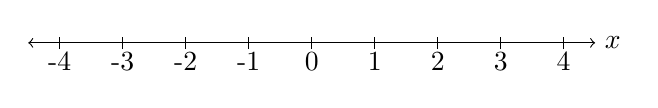
\begin{tikzpicture}[scale=0.8]
        \draw[<->] (-4.5,0) -- (4.5,0) node[right] {$x$};
        \foreach \x in {-4,-3,-2,-1,0,1,2,3,4} {
            \draw (\x, -0.1) -- (\x, 0.1);
            \node at (\x, -0.3) {\x};
        }
    \end{tikzpicture}
    \caption{បន្ទាត់ចំនួនបង្ហាញពីទីតាំងនៃចំនួនគត់។}
    \label{fig:integer-number-line}
\end{figure}

\section{ឧទាហរណ៍អនុវត្ត}

\begin{example}{ការប្រៀបធៀបចំនួនគត់}
តើមួយណាធំជាង, $-5$ ឬ $-2$?
\begin{solution}
នៅលើបន្ទាត់ចំនួន, $-2$ នៅខាងស្តាំ $-5$, ដូច្នេះ $-2 > -5$។
\end{solution}
\end{example}

\section{លំហាត់អនុវត្ត}
\begin{enumerate}[label=\arabic*.]
    \item ប្រៀបធៀប៖ $-10$ និង $1$។
    \item គណនា៖ $(-3) + 5$។
\end{enumerate}

